\documentclass{article}
\usepackage{amsfonts}
\usepackage{amsthm}
\usepackage{amssymb}
\usepackage{amsmath}
\usepackage{graphicx}
\usepackage{subcaption}
\usepackage{xcolor}

\newcommand{\new}[1]{
    \vspace{2mm}
    \noindent
    \textbf{
    \underline{#1}}
}

\def\calO{{\mathcal{O}}}
\def\th{{\theta}}
\def\_{{\hspace{1mm}}}
\def\<{{\langle}}
\def\>{{\rangle}}


\newcounter{problemcnt}
\setcounter{problemcnt}{0}

\newcommand{\Problem}{{
    \vspace{5mm}
    \stepcounter{problemcnt}
    \noindent
    \arabic{problemcnt}. 
}
}

\newcommand{\nProblem}[1]{
    \vspace{5mm}
    \noindent
    \setcounter{problemcnt}{#1}
    \arabic{problemcnt}. 
}


\newcommand{\Proof}{{
    \vspace{2mm}
    \noindent
    \textbf{
    \underline{Proof}}
}
}

\newcommand{\textOr}{
    {
        \hspace{5mm}
        \textrm{or}
        \hspace{5mm}
    }
}

\newcommand{\textAnd}{
    {
        \hspace{5mm}
        \textrm{and}
        \hspace{5mm}
    }
}

\newcommand{\halfFigure}[1]{
\begin{center}
\includegraphics[width = .5\linewidth]{{#1}}
\end{center}
}

\newcommand{\fullFigure}[2]{
\begin{center}
\includegraphics[width = .9\linewidth]{{#1}}
\end{center}
}

\def\twobytwoMat(#1, #2, #3, #4){
    {
        \begin{bmatrix}
            {#1} & {#2}\\
            {#3} & {#4}
        \end{bmatrix}
    }
}

\def\twobyoneMat(#1, #2){
    {
        \begin{bmatrix}
            {#1}\\
            {#2}
        \end{bmatrix}
    }
}

\def\twobytwoDet(#1, #2, #3, #4){
    {
        \begin{vmatrix}
            {#1} & {#2}\\
            {#3} & {#4}
        \end{vmatrix}
    }
}



\begin{document}
\begin{center}
\LARGE
PHYS 202 HW4

\Large
Daniel Son
\end{center}

\normalsize 


\new{Q1} 
Two masses $m_1, m_2$ are connected by a spring with a spring constant 
$k$. 

a) Write out a general solution for the position of the two masses. 

b) Find a specific solution for $x_1(0) = x_2(0) = 0$ and $v_1(0) = v$

c) Sketch $x_1(t)$ and $x_2(t)$. 


\new{Solution}

Each of the masses must have a linear term which 
describes the constant velocity of the center of mass. 
Also, each mass must have a oscillating term. By Newton's 2nd law, 
we write 

\[
    \ddot{x_1} = - k(x_1 - x_2) \textAnd 
    \ddot{x_2} = - k(x_2 - x_1)
\]

Also, in light of our previous observation, we guess the solution 
to be in the form of 
\[
    x_1 = Re[Ae^{i\omega t} + Ct]
    x_2 = Re[Be^{i \omega t} + Ct]
\]
It is possible to include a constant term, but it is possible to 
redefine $x_1, x_2$ to be zero at the defined place of axis, so 
we discard the extra variables for simplicity. 

Complexify the equation and plug them into the coupled differential 
eqation. 
We obtain the following matrix equation. 

\[
    k\twobytwoMat(-1/m_1, 1/m_1, 1/m_2, -1/m_2) \twobyoneMat(A, B) 
    = -\omega ^2 \twobyoneMat(A, B)
    \textOr 
    k\twobytwoMat(1/m_1, -1/m_1, -1/m_2, 1/m_2) \twobyoneMat(A, B) 
    = \omega ^2 \twobyoneMat(A, B)
\]



The eigensystem of the 2x2 matrix narrows down the candidates 
of the angular frequency and the amplitude $A, B$. According 
to mathematica, the eigensystem is as follows. 

\begin{center}
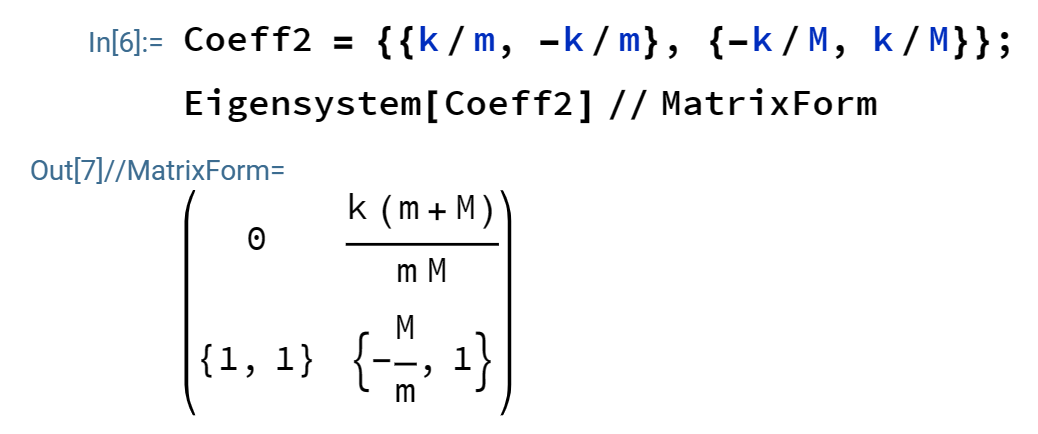
\includegraphics[width = .5\linewidth]{Fig1.png}
\end{center}

Thus, we obtain the two possible solutions. 
\[
    (\omega, A, B) = (0, G, G) \textOr (\sqrt{\frac{k(m+M)}{mM}}, -MG/m, G)
\]
Where $G$ is an arbitrary constant. The two restrictions 
does not provide constraints on $C$. 
Also, we defined the initial position to be zero at $t = 0$. 
Thus, we compute the imaginary part of the complexified equation 
instead of the real part. 
We write the general solution 
as follows. 

\[
    \boxed{
    (x_1, x_2) = (Ct, Ct) 
    \textOr 
    (-\frac{MG}{m}\sin(\sqrt{\frac{k(m+M)}{mM}} t)+ Ct, G\sin(\sqrt{\frac{k(m+M)}{mM}} t)+ Ct)
    }
\]


We simplify the equation by using the definition of reduced mass. 
\[
    \mu := \frac{mM}{m + M}
\]

\[
    \boxed{
    (x_1, x_2) = (Ct, Ct) 
    \textOr 
    (-\frac{MG}{m}\sin(\sqrt{k/ \mu} t)+ Ct, G\sin(\sqrt{k/\mu} t)+ Ct)}
\]

The center of mass mode cannot satisfy the given initial condition
To compute the particular solution, compute the time derivative 
of $x1$ and apply the condition $\dot{x_1}(0) = v, \dot{x_2}(0) = 0$. 

\[
    \dot{x_1}(0) = - \frac{MG}{m} \sqrt{\frac{k}{m}}+C = v \textAnd
    \dot{x_2}(0) = G \sqrt{k / \mu} + C = 0
\]

By subtracting each equation from one another, we derive an expression 
for $G$ and $C$. 

\[
    G = -\frac{v}{M} \sqrt{\frac{\mu^3}{k}}
    \textAnd 
    C = v\frac{\mu}{M}
\]

Plugging in, we obtain
\[
    \boxed{
    (x_1, x_2) = \biggl(
        \frac{v}{m} \sqrt{\mu^3/k} \sin (\sqrt{k/\mu} t) + \frac{v \mu} {M} t
        ,
        -\frac{v}{M} \sqrt{\mu^3/k} \sin (\sqrt{k/\mu} t) + \frac{v \mu} {M} t
    \biggr)
    }
\]

\new{Q2}
Find the normal modes of a two-body oscillator that is 
vertically attatched to a ceiliing. 

\new{Solution}
Let $x_1, x_2$ be the displacement from the equilibrium positon of the two masses. 
Gravity can be ignored by considering the equilibrium position. 
Writing out the force eqution in matrix form 
\[
    m\frac{d^2}{dt^2}\twobyoneMat(x_1, x_2)
    = 
    -k \twobytwoMat(2, -1, -1, 1) \twobyoneMat(x_1, x_2)
\]
Assuming a solution in the form of $x = e^{i\omega t}$, 
$\omega^2$ will be the eigenvalues of the matrix 
\[
    \frac{k}{m} \twobytwoMat(2, -1, -1, 1)
\]. The eigenvalues will correspond to the amplitude of 
the two displacements. 

\halfFigure{Fig6}

Thus, the two frequencies of the normal modes are 
\[
    \sqrt{
        \frac{(3 + \sqrt{5})k}{2m}
    }
    , 
    \sqrt{
        \frac{(3 - \sqrt{5})k}{2m}
    }
\]

And the first frequency is the higher frequency and 
the second frequcncy is the lower frequency. For the 
higher frequency, the two masses move in the opposite 
direction, and the top mass moves at a greater amplitude. 
For the lower frequency, the two masses move in the same 
direction, and the top mass moves with less magnitude. 

\hfill \qed



\new{Q3} Asymmetric strings

a) Set up equations and find the matrix whose eigenvalues can be related to normal mode 
frequencies

\new{Solution}

Let $x_1, x_2$ denote the equilibrium position of the two masses. 
By Newton's 2nd law 
\[
    m\ddot{x_1} = -k_1x_1-k_C(x_1-x_2)
    \textAnd
    m\ddot{x_2} = -k_2x_2-k_C(x_2 - x_1)  
\]
Dividing my masses
\[
    \ddot{x_1} = -\omega _1^2x_1-\omega_C^2(x_1-x_2)
    \textAnd
    \ddot{x_2} = -\omega _2^2x_2-\omega_C^2(x_2 - x_1)  
\]
Complexify the equations, and try solutions in the form of 
$(x_1, x_2) = (Ae^{-i\omega t}, Be^{i \omega t})$. 
By plugging in the equation and dividing by the exponential 
term, we obtain 

\[
    \twobytwoMat(-\omega_C^2 - \omega_1^2, 
    \omega_C^2,
    \omega_C^2,
    -\omega_C^2 - \omega_2^2) 
    \twobyoneMat(A, B) = 
    -\omega^2 \twobyoneMat(A, B)
\]

Multiply both sides by negative one. 


\[
    \twobytwoMat(\omega_C^2 +\omega_1^2, 
    -\omega_C^2,
    -\omega_C^2,
    \omega_C^2 +\omega_2^2) 
    \twobyoneMat(A, B) = 
    \omega^2 \twobyoneMat(A, B)
\]

Collect $\omega_1^2$ from the LHS, and divide by it both sides.  

\[
    \twobytwoMat(\beta + 1, -\beta, -\beta, \beta + \alpha) 
    \twobyoneMat(A, B) = 
    (\omega/\omega_1)^2 \twobyoneMat(A, B)
\]

The eigensystem of the coefficient matrix above will yield 
the value of $(\omega/\omega_1)^2$ and its corresponding 
eigenvectors. The following mathematica code shows the result.

\begin{center}
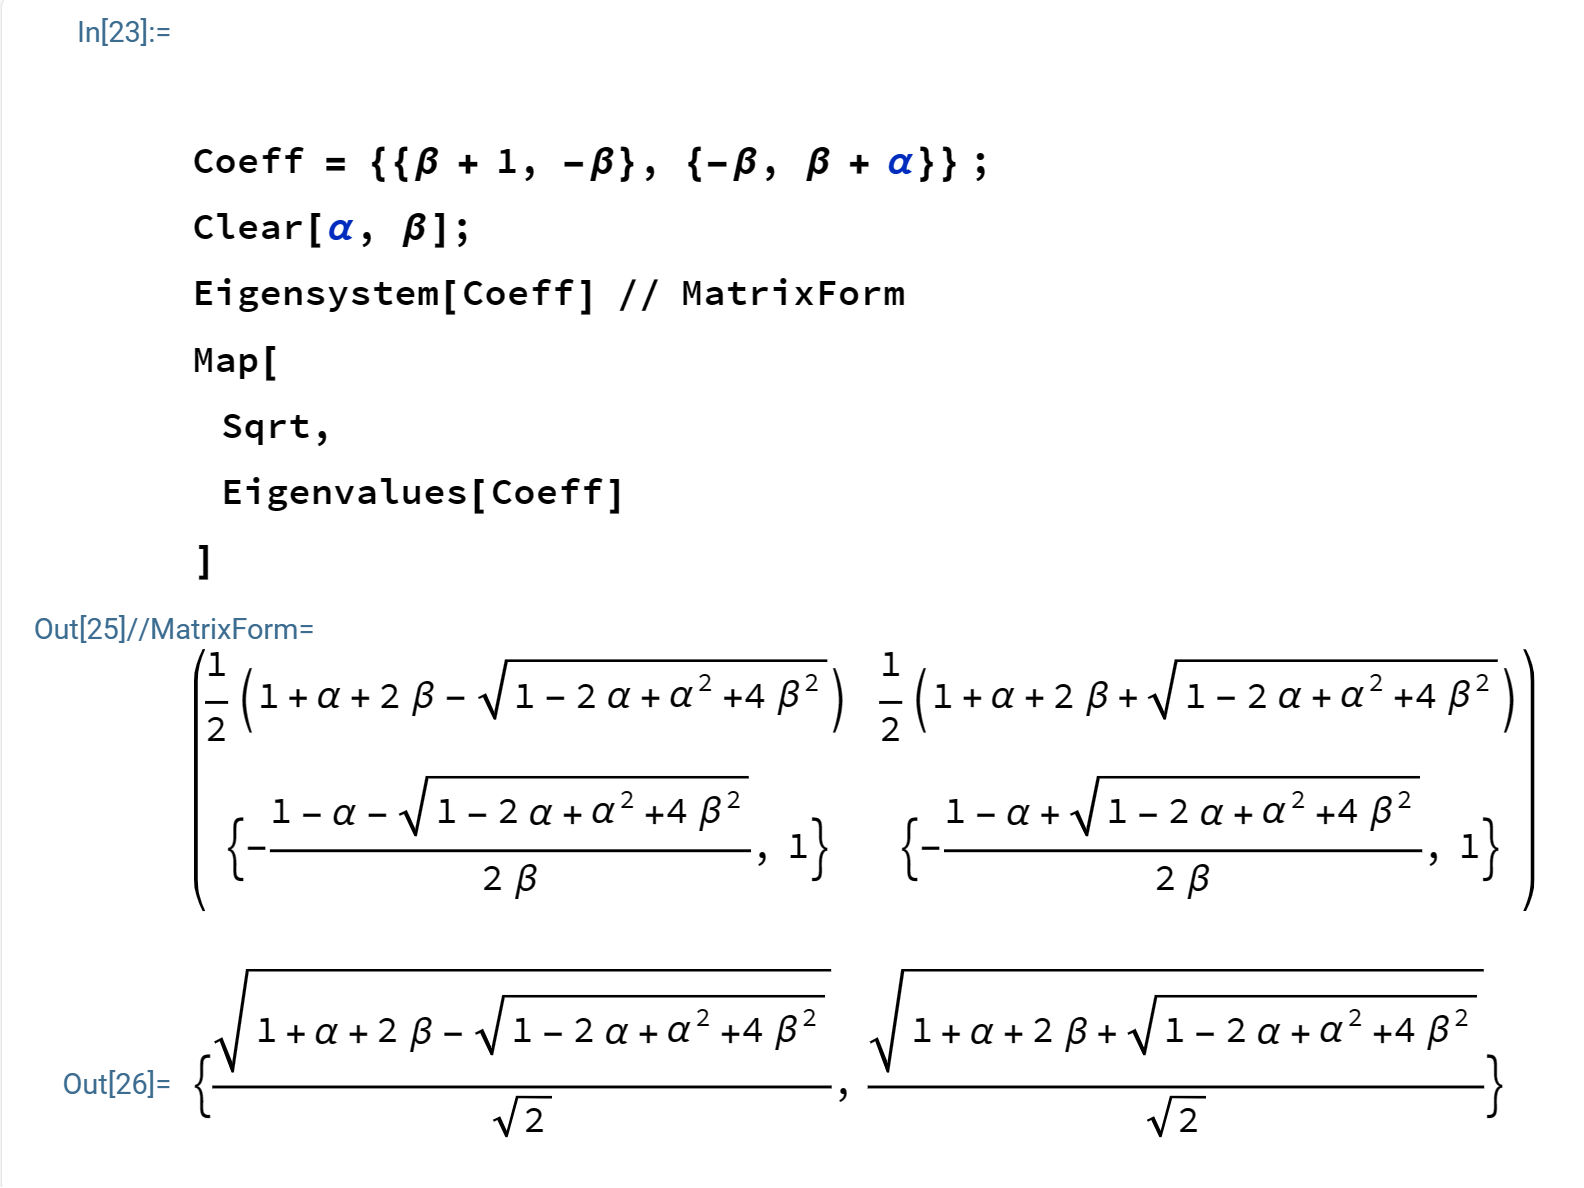
\includegraphics[width = .9\linewidth]{Fig2.png}
\end{center}


Plugging in $\alpha = 1$, the eigensystem simplies as follows. 

\begin{center}
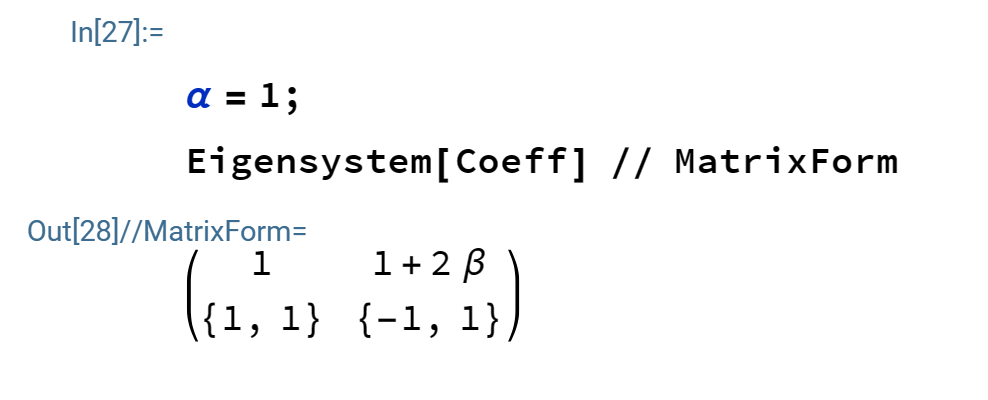
\includegraphics[width = .5\linewidth]{Fig3.png}
\end{center}

So for the $\alpha = 1$ case, we confirm that 
$\omega/\omega_1 = 1$ results in the center of 
mass mode, and $\omega/\omega_1 = \sqrt{1+2\beta}$ 
results in the breathing mode. $\alpha = 1$ means that 
the string constant of the two strings connected to 
the wall are identical, and the eigenvectors concur 
with the physical phenomena. 

Now, apply the taylor approximation on both of the resonant 
frequencies. Call them $\omega_s, \omega_f$ respectively. For 
real values $x, y$ where $y \ll 1$, we have an approximation 
\[
    \sqrt{x+y} \approxeq \sqrt{x} + \frac{y}{2\sqrt{x}}
\]. 


Applying this approximation, 

\[
    \xi := \sqrt{(1-a)^2 + 4\beta^2} 
    \approxeq (1-\alpha) + 2\frac{\beta^2}{1-\alpha}
    \approxeq (1-\alpha)
\]

and also,
\[
    \omega_s = \frac{
        \sqrt{1 + \alpha + 2\beta - \xi}
    }{\sqrt{2}}
    \approxeq 
    \sqrt{
        \frac{1 + \alpha + 2\beta - (1 - \alpha)}{2}
    }
    =
        \sqrt{
            \alpha + \beta
        }
    \approxeq 
    \sqrt{\alpha} + \frac{\beta}{2\sqrt{\alpha}}
\]
\[
    \omega_f = \frac{
        \sqrt{1 + \alpha + 2\beta + \xi}
    }{\sqrt{2}}
    \approxeq 
    \sqrt{
        \frac{1 + \alpha + 2\beta + (1 - \alpha)}{2}
    }
    =
        \sqrt{
            1 + \beta
        }
    \approxeq 
    1 + \frac{\beta}{2}
\]
To sum up 
\[
    \boxed{
    (\omega_s, \omega_f)
    = 
    (
    \sqrt{\alpha} + \frac{\beta}{2\sqrt{\alpha}}
    ,
1 + \frac{\beta}{2}
    )
    }
\]
\textbf{Remark} If $\alpha > 1$, then the signs of $\xi$ swap. 
The abve equation is correct for $\alpha \ll 1$, but for $\alpha \gg 1$, 
$\omega_s$ and $\omega_f$ must be swapped. 

\fullFigure{Fig4}

\fullFigure{Fig7}

\fullFigure{Fig5}

\new{Solution 1} Using impedences 

Use Newton's second law to write out the 
equations that govern the movement of the mechanical oscillator. 
    \begin{align*}
        m\ddot{x_1} &= -k(x_1-x_2)\\
        m\ddot{x_2} &= -k(x_2 - x_1) - k(x_2 - x_3)\\
        m\ddot{x_3} &= -k(x_3-x_2)
    \end{align*}

For convinience, manipulate the second equation in the form 
\[
  \ddot{x_2}  =    -\ddot{x_1} - \ddot{x_3}
\]

As for the RLC circuit, define the circuit direction to point 
from bottom to the top, and call the currents $I_1, I_2, I_3$
from left to right. The voltage through each of the three 
paths must be conserved by the loop rule. Complexifying 
the currents and applying the complex version of Ohm's law, 
we write 

\[
    \tag{1}
    \tilde{I_1}(\frac{1}{i\omega C} + i\omega L) 
    = \tilde{I_2} \frac{1}{i\omega C}
    = \tilde{I_3} (\frac{1}{i\omega C} + i\omega L)
\]

The solution of the currents will be in the form $\tilde{I} = Ae^{i\omega t}$. 
We deduce 
\[ 
    i\omega \tilde{I} = \frac{d}{dt}\tilde{I} = \ddot{\tilde{Q}}
    \textAnd 
    \frac{\tilde{I}}{i\omega} = \tilde{Q}
\]

Where $\ddot{Q}$ is the complexified charge of any capacitor. 
The script is omitted to imply that the rule applies to all 
capacitors in the circuit. 

In light of this identity, rewrite (1) in terms of charge. 

\[
    \frac{1}{C}\tilde{Q_1}+L\ddot{\tilde{Q_1}}
    = 
    \frac{1}{C}\tilde{Q_2}
    = 
    \frac{1}{C}\tilde{Q_3} + L\ddot{\tilde{Q_3}}
\]

Call each side of the equation $A, B, C$. Rewriting 
$A = B , C = B $, we obtain 
\[
    L\ddot{\tilde{Q_1}} = \frac{1}{C}(\tilde{Q_2} - \tilde{Q_1})
    \tag{a}
\]
\[
    L\ddot{\tilde{Q_3}} = \frac{1}{C}(\tilde{Q_3} - \tilde{Q_1})
    \tag{b}
\]
Finally, by applying the junction rule on the top center junction, 
\[
    \dot{Q_1} + \dot{Q_2} + \dot{Q_3} = 0
\]
and differentiating by time and with some manipulation 
\[
    \ddot{Q_2} = -\ddot{Q_1}-\ddot{Q_3}
    \tag{c}
\]

Indeed, the isomorphism $(k, m) \mapsto (1/C, L)$ 
verifies that the equations a, b, c are indeed isomorphic 
to the equations of the mechanical system. 

\qed


\new{Q5} Describe the normal modes of the CO2 molecule. 

\new{Solution}
We start with deriving the normal mode frequencies. 
Consider the molecules as three masses located 
at equilibrium position $x_1, x_2, x_3$. Their respective 
masses will be $m_O, m_C, m_O$ respectively. For 
convinience, define the vector $\vec{x} := (x_1, x_2, x_3)$. 
By Newton's 2nd law, 
\[
    M\frac{d^2}{dt^2} \vec{x} = -K \vec{x}
    \tag{1}
\]
Where the matricies $M, K$ is 
\[
    M := diag\{m_O, m_C, m_O\}, K:=-k
    \begin{bmatrix}
        1 & -1 & 0\\
        -1 & 2 & -1\\
        0 & -1 & 1
    \end{bmatrix}
\]

The inverse of a diagonal matrix can also be 
written as a diagonal matrix where each entry is the 
reciprocal of the original entry. From (1), multiply 
both sides by $M^{-1}$ to the left. 

\[
    \frac{d^2}{dt^2}\vec{x} = -M^{-1}K \vec{x}
=
diag\{1/m_O, 1/m_C, 1/m_O\} (-k) K \vec{x}
    \]

Multiplying by the diagonal matrix on the left results in 
each column being multiplied by the corresponding entry. Also, 
pull out the scalar $1/m_O$. 

\[
    \boxed{
    \frac{d^2}{dx^2}\vec{x} = 
    -\frac{k}{m_O} diag\{1, 4/3, 1\} K\vec{x} 
    = 
-\frac{k}{m_O}
 \begin{bmatrix}
        1 & -1 & 0\\
        -4/3 & 8/3 & -4/3\\
        0 & -1 & 1
    \end{bmatrix}
    \vec{x}
    }
\]

For convinience, we define 
\[
    C := \begin{bmatrix}
        3& -3& 0\\ 
        -4 & 8 & -4 \\
        0 & -3 & 3
    \end{bmatrix}
\]
We wish to compute the eigenvalues and the eigevectors 
that correlate to $M^{-1}K = -\frac{k}{3m_O} C$. We compute 
these quantities for $C$ and make adjustments. 

The characteristic polynomial of $C$ is 
\[
    |C - \lambda I| = \begin{vmatrix}
        3- \lambda& -3& 0\\ 
        -4 & 8 - \lambda& -4 \\
        0 & -3 & 3 - \lambda
    \end{vmatrix}
    = (3 - \lambda)(\lambda - 8)\lambda
\]

The spectrum i.e. the set of eigenvalues of $C$ is 
${0, 3, 8}$. We derive the corresponding eigenvectors 
by computing the nullspace of $C - \lambda I$. 

With some algebra, we conclude that the eigensystem of $C$
to be as follows. 

\begin{align*}
    \lambda = 0 \mapsto (1, 1, 1) \\
    \lambda = 3 \mapsto (1, 0, -1) \\ 
    \lambda = 8 \mapsto (3, -8, 3)
\end{align*}

Thus, the eigensystem of the matrix $M^{-1}K = -\frac{k}{3m_O} C$
is 
\begin{align*}
    \lambda = 0 &\mapsto (1, 1, 1) \\
    \lambda = -\frac{k}{m_O}&\mapsto (1, 0, -1) \\ 
    \lambda = -\frac{8k}{3m_O} &
\mapsto (3, -8, 3)
\end{align*}

From top to bottom, each mode corresponds to the center of mass mode, 
breathing mode, and the egyptian mode. \qed


\end{document}